%% TODO show that all the stated equivalence relations are actually eq. rel.s
\begin{theorem}$R_{eq} \subsetneq R_{bc} \subsetneq R_{par}$\end{theorem}
\begin{proof}
  Let $(x, y)\in R_{eq}$, so $x=y$. Then $x$ has exactly the same number of ones
  as $y$ (and the same number of zeros, and in the same order), so $(x, y) \in
  R_{bc}$. Therefore, $R_{eq} \subset R_{bc}$.
 
  Consider $x=1100$ and $y=0101$. Then $(x, y)\in R_{bc}$ but $(x, y) \notin
  R_{eq}$. Therefore $R_{eq} \neq R_{bc}$.

  Let $(x, y)\in R_{bc}$, so $x$ and $y$ have the same number of ones. Let $k$
  be the number of ones in $x$, and $l$ be the number of ones in $y$. Then
  $l=k$, which implies $l \equiv k$ (mod 2). Therefore $x$ and $y$ have
  the same parity, so $(x, y)\in R_{par}$. Therefore $R_{bc} \subset R_{par}$.

  Consider $x=1000$ and $y=1011$. Then $(x, y)\in R_{par}$ but $(x, y) \notin
  R_{bc}$. Therefore $R_{bc} \neq R_{par}$.
\end{proof}

\begin{theorem}$R_{eq} \subsetneq R_{eqi}$\end{theorem}
\begin{proof}
  Let $(x, y)\in R_{eq}$, so $x=y$. Then $(x, y)$ satisfies the property
  specified in the definition of $R_{eqi}$, specifically that $x=y$, so
  $(x, y) \in R_{eqi}$. Therefore $R_{eq} \subset R_{eqi}$.

  Consider $x=1000$ and $y=0111$. Then $(x, y)\in R_{eqi}$ but $(x, y) \notin
  R_{eq}$. Therefore $R_{eq} \neq R_{eqi}$.
\end{proof}

\autoref{fig:containments} exhibits the containments among $R_{eq}$, $R_{eqi}$,
$R_{bc}$, and $R_{par}$. Note that if $a=0^n$, for $n=|x|=|y|$, then
$R_{a}=R_{eq}$ and if $a=1^n$ then $R_{a}=R_{eqi}$.

Since membership in $R_{par}$, $R_{bc}$, $R_{eq}$, $R_{eqi}$, and $R_a$ can be
decided in polynomial time, so they are all members of \PEq.

\begin{figure}
  \begin{center}
    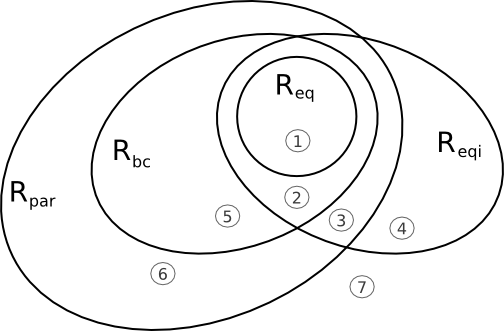
\includegraphics[width=300pt,height=241pt,keepaspectratio=true]
                    {containments.png}
  \end{center}
  \caption{ \label{fig:containments} Containment relationships for equivalence
    relations $R_{eq}$, $R_{eqi}$, $R_{bc}$, and $R_{par}$. The following are
    example elements in the sets at the specified locations: 1. (1100, 1100)
    2. (1010, 0101) 3. (1000, 0111) 4. (10000, 01111) 5. (1000, 0001) 6. (1000,
    1011) 7. (1000, 0000) }
\end{figure}
